\documentclass[tikz]{standalone}
\usepackage{tikz}
\usepackage{fourier}
\usepackage{physics}
\usetikzlibrary{shapes.geometric}
\usetikzlibrary{calc}

\begin{document}

\begin{tikzpicture}
    % First row
    \node at (0, 0) {\(\zeta={(1, 0, 0, 0, 0)}^T\)};
    \node at (4.5, 0) {\(\zeta={(0, 1, 0, 0, 0)}^T\)};
    \node at (9, 0) {\(\zeta={(0, 0, 1, 0, 0)}^T\)};

    \node at (0, -1.8){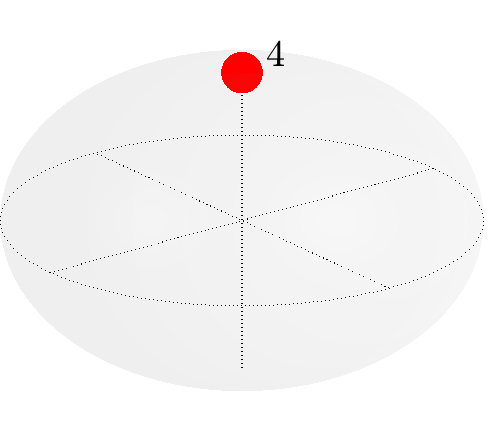
\includegraphics[width=0.3\textwidth]
    {gfx/FM-2-Majorana.pdf}};
    \node at (4.5, -1.8){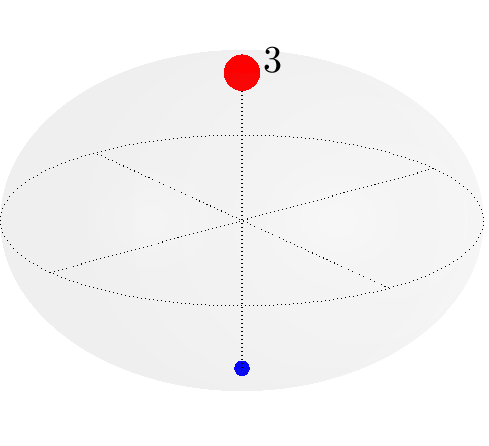
\includegraphics[width=0.3\textwidth]
    {gfx/FM-1-Majorana.pdf}};
    \node at (9, -1.8){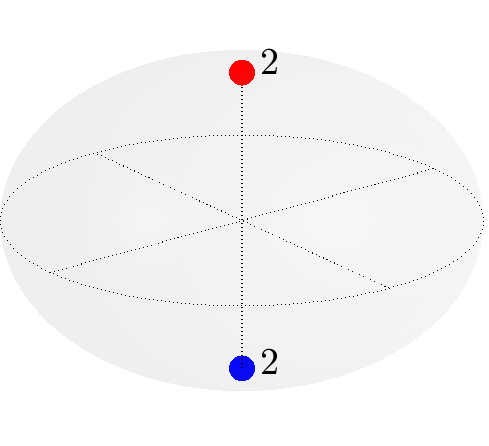
\includegraphics[width=0.3\textwidth]
    {gfx/UN-Majorana.pdf}};
        
    \node at (0, -3.5) {(a)};
    \node at (4.5, -3.5) {(b)};
    \node at (9, -3.5) {(c)};
    
    % Second row
    \node at (0, -4) {\(\zeta={(1, 0, 0, 0, 1)}^T/\sqrt{2}\)};
    \node at (4.5, -4) {\(\zeta={(1, 0, i\sqrt{2}, 0, 1)}^T/2\)};
    \node at (9, -4) {\(\zeta={(\sqrt{1/3}, 0, 0, \sqrt{2/3}, 0)}^T\)};

    \node at (0, -5.8){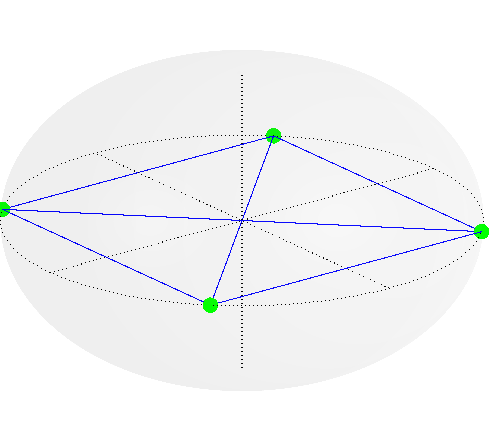
\includegraphics[width=0.3\textwidth]
    {gfx/BN-Majorana.pdf}};
    \node at (4.5, -5.8){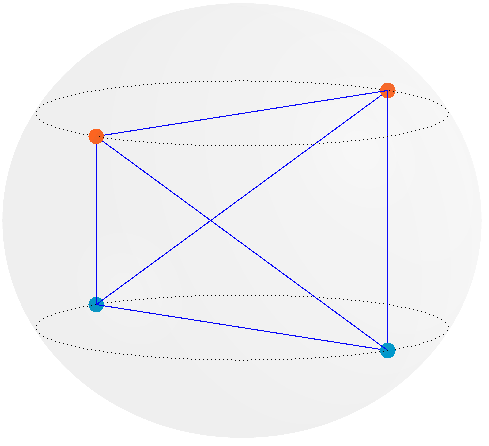
\includegraphics[width=0.265\textwidth]
    {gfx/C1-Majorana.pdf}};
    \node at (9, -5.8){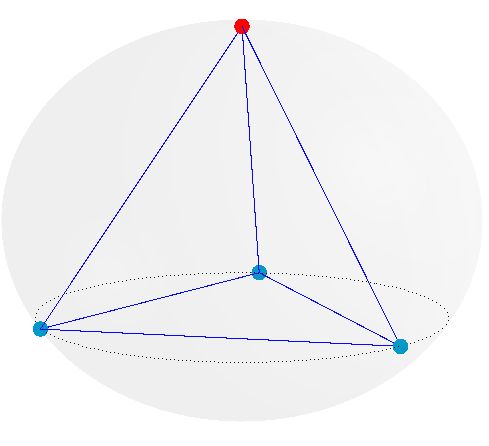
\includegraphics[width=0.275\textwidth]
    {gfx/C2-Majorana.pdf}};
    
    \node at (0, -7.6) {(d)};
    \node at (4.5, -7.6) {(e)};
    \node at (9, -7.6) {(f)};
    
    % Colour bar
    \node at (11.8, -3.5) {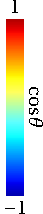
\includegraphics{gfx/compiled_jet_majorana.pdf}};
\end{tikzpicture}
\end{document}